\chapter{Bayesian Statistics}\label{chapter:Bayes}\index{general}{Bayesian Statistics}

\section{Bayesian vs. Frequentist Interpretation}

Calculating probabilities is only one part of statistics. Another is the interpretation of them - and the consequences that come with different interpretations.

So far we have restricted ourselves to the \emph{frequentist interpretation}\index{general}{interpretation!frequentist}, which interprets $p$ as the \emph{frequency of an occurrence}: if an outcome of an experiment has the probability $p$, it means that if that experiment is repeated $N$ times (where $N$ is a large number), then we observe this specific outcome $N*p$ times.

The \emph{Bayesian interpretation}\index{general}{interpretation!Bayesian} of $p$ is quite different, and interprets $p$ as our \emph{believe of the likelihood} of a certain outcome. For some events, this makes a lot more sense. For example, in the upcoming semi-final of the soccer worldcup in Brazil, Argentine will play against the Netherlands, with Lionel Messi leading the Argentinian team. Since Messi is (for a soccer player) already fairly old, this may be a one-time event, and we will never have a large number $N$ repetitions.

But in addition to this difference in interpretation, the Bayesian approach has another advantage: it lets us bring in \emph{prior knowledge} into the calculation of the probability $p$, through the application of \emph{Bayes' Theorem}\index{general}{Bayes' Theorem}:

In its most common form, it is:

\begin{equation}\label{eq:BayesTheorem}
  P(A|B) = \frac{P(B | A)\, P(A)}{P(B)}\cdot
\end{equation}

In the Bayesian interpretation, probability measures a degree of belief. Bayes's theorem then links the degree of belief in a proposition before and after accounting for evidence. For example, suppose it is believed with 50\% certainty that a coin is twice as likely to land heads than tails. If the coin is flipped a number of times and the outcomes observed, that degree of belief may rise, fall or remain the same depending on the results.

John Maynard Keynes, a great economist and thinker, said "When the facts change, I change my mind. What do you do, sir?" This quote reflects the way a Bayesian updates his or her beliefs after seeing evidence.

For proposition A and evidence B,

\begin{itemize}
  \item P(A), the \emph{prior probabiliby}\index{general}{prior probability}, is the initial degree of belief in A.
  \item P(A|B), the \emph{posterior probability}\index{general}{posterior probability}, is the degree of belief having accounted for B. It can be read as \emph{"the probability of A, given that B is the case"}.
  \item the quotient P(B|A)/P(B) represents the support B provides for A.
\end{itemize}

If the number of available data points is large, the difference in interpretation does typically not change the result significantly. If the number of data points is small, however, the possibility to bring in external knowledge may lead to a significantly improved estimation of $p$.

\subsection{Bayesian Example}

\footnote{This example, and the above definition of Bayes' Theorem, has been taken from Wikipedia}Suppose a man told you he had a nice conversation with someone on the train. Not knowing anything about this conversation, the probability that he was speaking to a woman is 50\% (assuming the speaker was as likely to strike up a conversation with a man as with a woman). Now suppose he also told you that his conversational partner had long hair. It is now more likely he was speaking to a woman, since women are more likely to have long hair than men. Bayes's theorem can be used to calculate the probability that the person was a woman.

To see how this is done, let W represent the event that the conversation was held with a woman, and L denote the event that the conversation was held with a long-haired person. It can be assumed that women constitute half the population for this example. So, not knowing anything else, the probability that W occurs is P(W) = 0.5.

Suppose it is also known that 75\% of women have long hair, which we denote as P(L |W) = 0.75 (read: the probability of event L given event W is 0.75, meaning that the probability of a person having long hair (event "L"), given that we already know that the person is a woman ("event W") is 75\%). Likewise, suppose it is known that 15\% of men have long hair, or P(L |M) = 0.15, where M is the complementary event of W, i.e., the event that the conversation was held with a man (assuming that every human is either a man or a woman).

Our goal is to calculate the probability that the conversation was held with a woman, given the fact that the person had long hair, or, in our notation, P(W |L). Using the formula for Bayes's theorem, we have:

\begin{equation*}
  P(W|L) = \frac{P(L|W) P(W)}{P(L)} = \frac{P(L|W) P(W)}{P(L|W) P(W) + P(L|M) P(M)}
\end{equation*}

where we have used the law of total probability to expand P(L). The numeric answer can be obtained by substituting the above values into this formula (the algebraic multiplication is annotated using "$\cdot$", the centered dot). This yields

\begin{equation*}
  P(W|L) = \frac{0.75\cdot0.50}{0.75\cdot0.50 + 0.15\cdot0.50} = \frac56\approx 0.83,
\end{equation*}

i.e., the probability that the conversation was held with a woman, given that the person had long hair, is about 83\%.

Another way to do this calculation is as follows. Initially, it is equally likely that the conversation is held with a woman as with a man, so the prior odds are 1:1. The respective chances that a man and a woman have long hair are 15\% and 75\%. It is 5 times more likely that a woman has long hair than that a man has long hair. We say that the likelihood ratio or Bayes factor is 5:1. Bayes's theorem in odds form, also known as Bayes's rule, tells us that the posterior odds that the person was a woman is also 5:1 (the prior odds, 1:1, times the likelihood ratio, 5:1). In a formula:

\begin{equation*}
  \frac{P(W|L)}{P(M|L)} = \frac{P(W)}{P(M)} \cdot \frac{P(L|W)}{P(L|M)}.
\end{equation*}

\section{The Bayesian Approach in the Age of Computers}

Bayes's theorem was named after the Reverend Thomas Bayes (1701 - 1761), who studied how to compute a distribution for the probability parameter of a binomial distribution. So it has been around for a long time. The reason Bayes' Theorem has become so popular in statistics in recent years is the cheap availability of massive computational power. This allows the empirical calculation of posterior probabilities, one-by-one, for each new piece of evidence. This, combined with statistical approaches like \emph{Markov Chain Monte Carlo (MCMC)} simulations, has allowed radically new statistical analysis procedures, and has led to what may be called "statistical trench warfare" between the followers of the different philosophies. If you don't believe me, check the corresponding discussions on the WWW.

For more information on that topic, check out (in order of rising complexity)

\begin{itemize}
  \item Wikipedia, which has some nice explanations under \emph{"Bayes ..."}
  \item \href{http://camdavidsonpilon.github.io/Probabilistic-Programming-and-Bayesian-Methods-for-Hackers/}{Bayesian Methods for Hackers}, a nice, free ebook, providing a practical introduction to the use of PyMC (see below).
  \item The \href{http://pymc-devs.github.io/pymc/}{PyMC User Guide}: PyMC is a very powerful Python package which makes the application of MCMC techniques very simple.
  \item \emph{Pattern Recognition and Machine Learning}, a comprehensive, but often quite technical book by Christopher M. Bishop \cite{Bishop2007}.
\end{itemize}

\section{Example: The Challenger Disaster}

This is an excerpt of the excellent 'Bayesian Methods for Hackers'. For the whole book, check out \href{http://camdavidsonpilon.github.io/Probabilistic-Programming-and-Bayesian-Methods-for-Hackers/}{Bayesian Methods for Hackers}.

On January 28, 1986, the twenty-fifth flight of the U.S. space shuttle program ended in disaster when one of the rocket boosters of the Shuttle Challenger exploded shortly after lift-off, killing all seven crew members. The presidential commission on the accident concluded that it was caused by the failure of an O-ring in a field joint on the rocket booster, and that this failure was due to a faulty design that made the O-ring unacceptably sensitive to a number of factors including outside temperature. Of the previous 24 flights, data were available on failures of O-rings on 23, (one was lost at sea), and these data were discussed on the evening preceding the Challenger launch, but unfortunately only the data corresponding to the 7 flights on which there was a damage incident were considered important and these were thought to show no obvious trend. The data are shown below:

\begin{figure}[H]
  \centering
  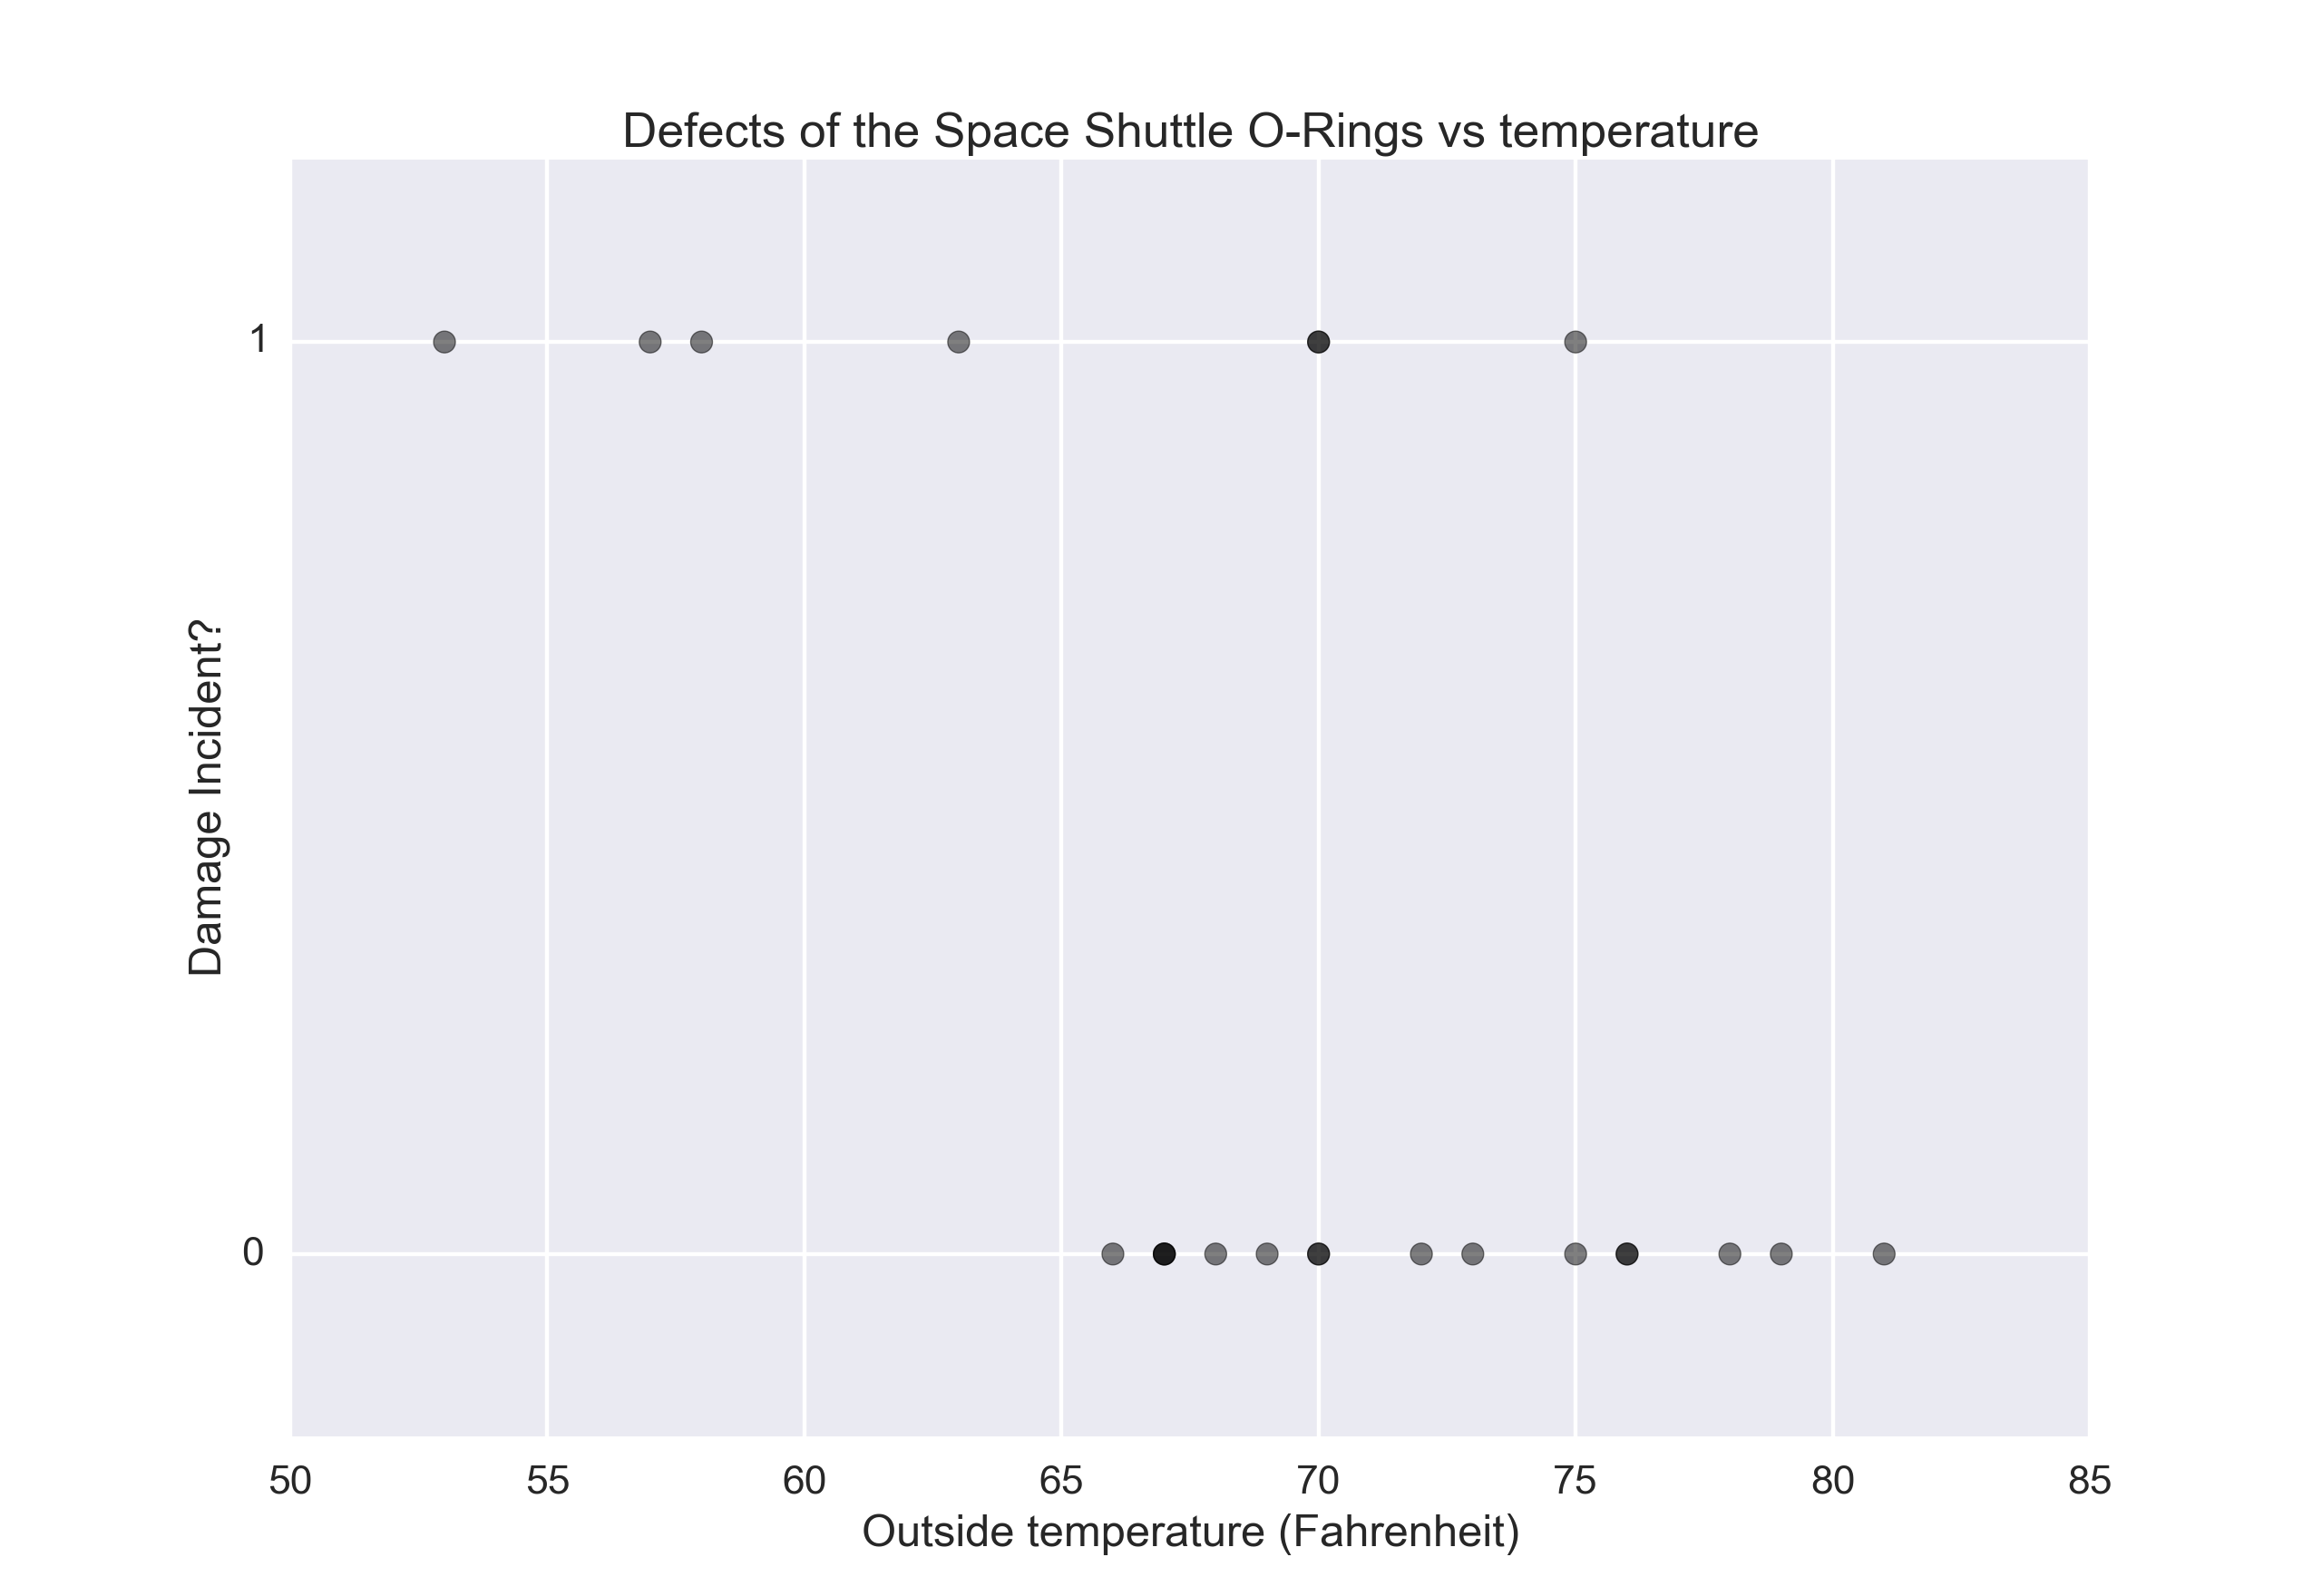
\includegraphics[width=0.5\textwidth]{../Images/Challenger_ORings.png}\\
  \caption{Failure of O-rings during space shuttle launches, as a function of temperature.}
\end{figure}

To simulate the probability of the O-rings failing, we need a function that goes from one to zero. One of the most frequently used functions for that is the \emph{logistic function}\index{general}{logistic function}:

\begin{equation}\label{eq:logisticFcn}
  p(t) = \frac{1}{ 1 + e^{ \;\beta t + \alpha } }
\end{equation}

In this model, the variable $\beta$ that describes how quickly the function changes from 1 to 0, and $\alpha$ indicates the location of this change.

Using the Python package PyMC, a Monte-Carlo simulation of this model can be done remarkably easily (Note: at the time of writing, PyMC was not yet released for Python 3!):

\begin{lstlisting}
    # --- Perform the MCMC-simulations ---
    temperature = challenger_data[:, 0]
    D = challenger_data[:, 1]  # defect or not?

    # Define the prior distributions for alpha and beta
    # 'value' sets the start parameter for the simulation
    # The second parameter for the normal distributions is the "precision",
    # i.e. the inverse of the standard deviation
    beta = pm.Normal("beta", 0, 0.001, value=0)
    alpha = pm.Normal("alpha", 0, 0.001, value=0)

    # Define the model-function for the temperature
    @pm.deterministic
    def p(t=temperature, alpha=alpha, beta=beta):
        return 1.0 / (1. + np.exp(beta * t + alpha))

    # connect the probabilities in `p` with our observations through a
    # Bernoulli random variable.
    observed = pm.Bernoulli("bernoulli_obs", p, value=D, observed=True)

    # Combine the values to a model
    model = pm.Model([observed, beta, alpha])

    # Perform the simulations
    map_ = pm.MAP(model)
    map_.fit()
    mcmc = pm.MCMC(model)
    mcmc.sample(120000, 100000, 2)
\end{lstlisting}

From this simulation, we obtain not only our best estimate for $\alpha$ and $\beta$, but also information about our uncertainty about these values:

\begin{figure}[H]
  \centering
  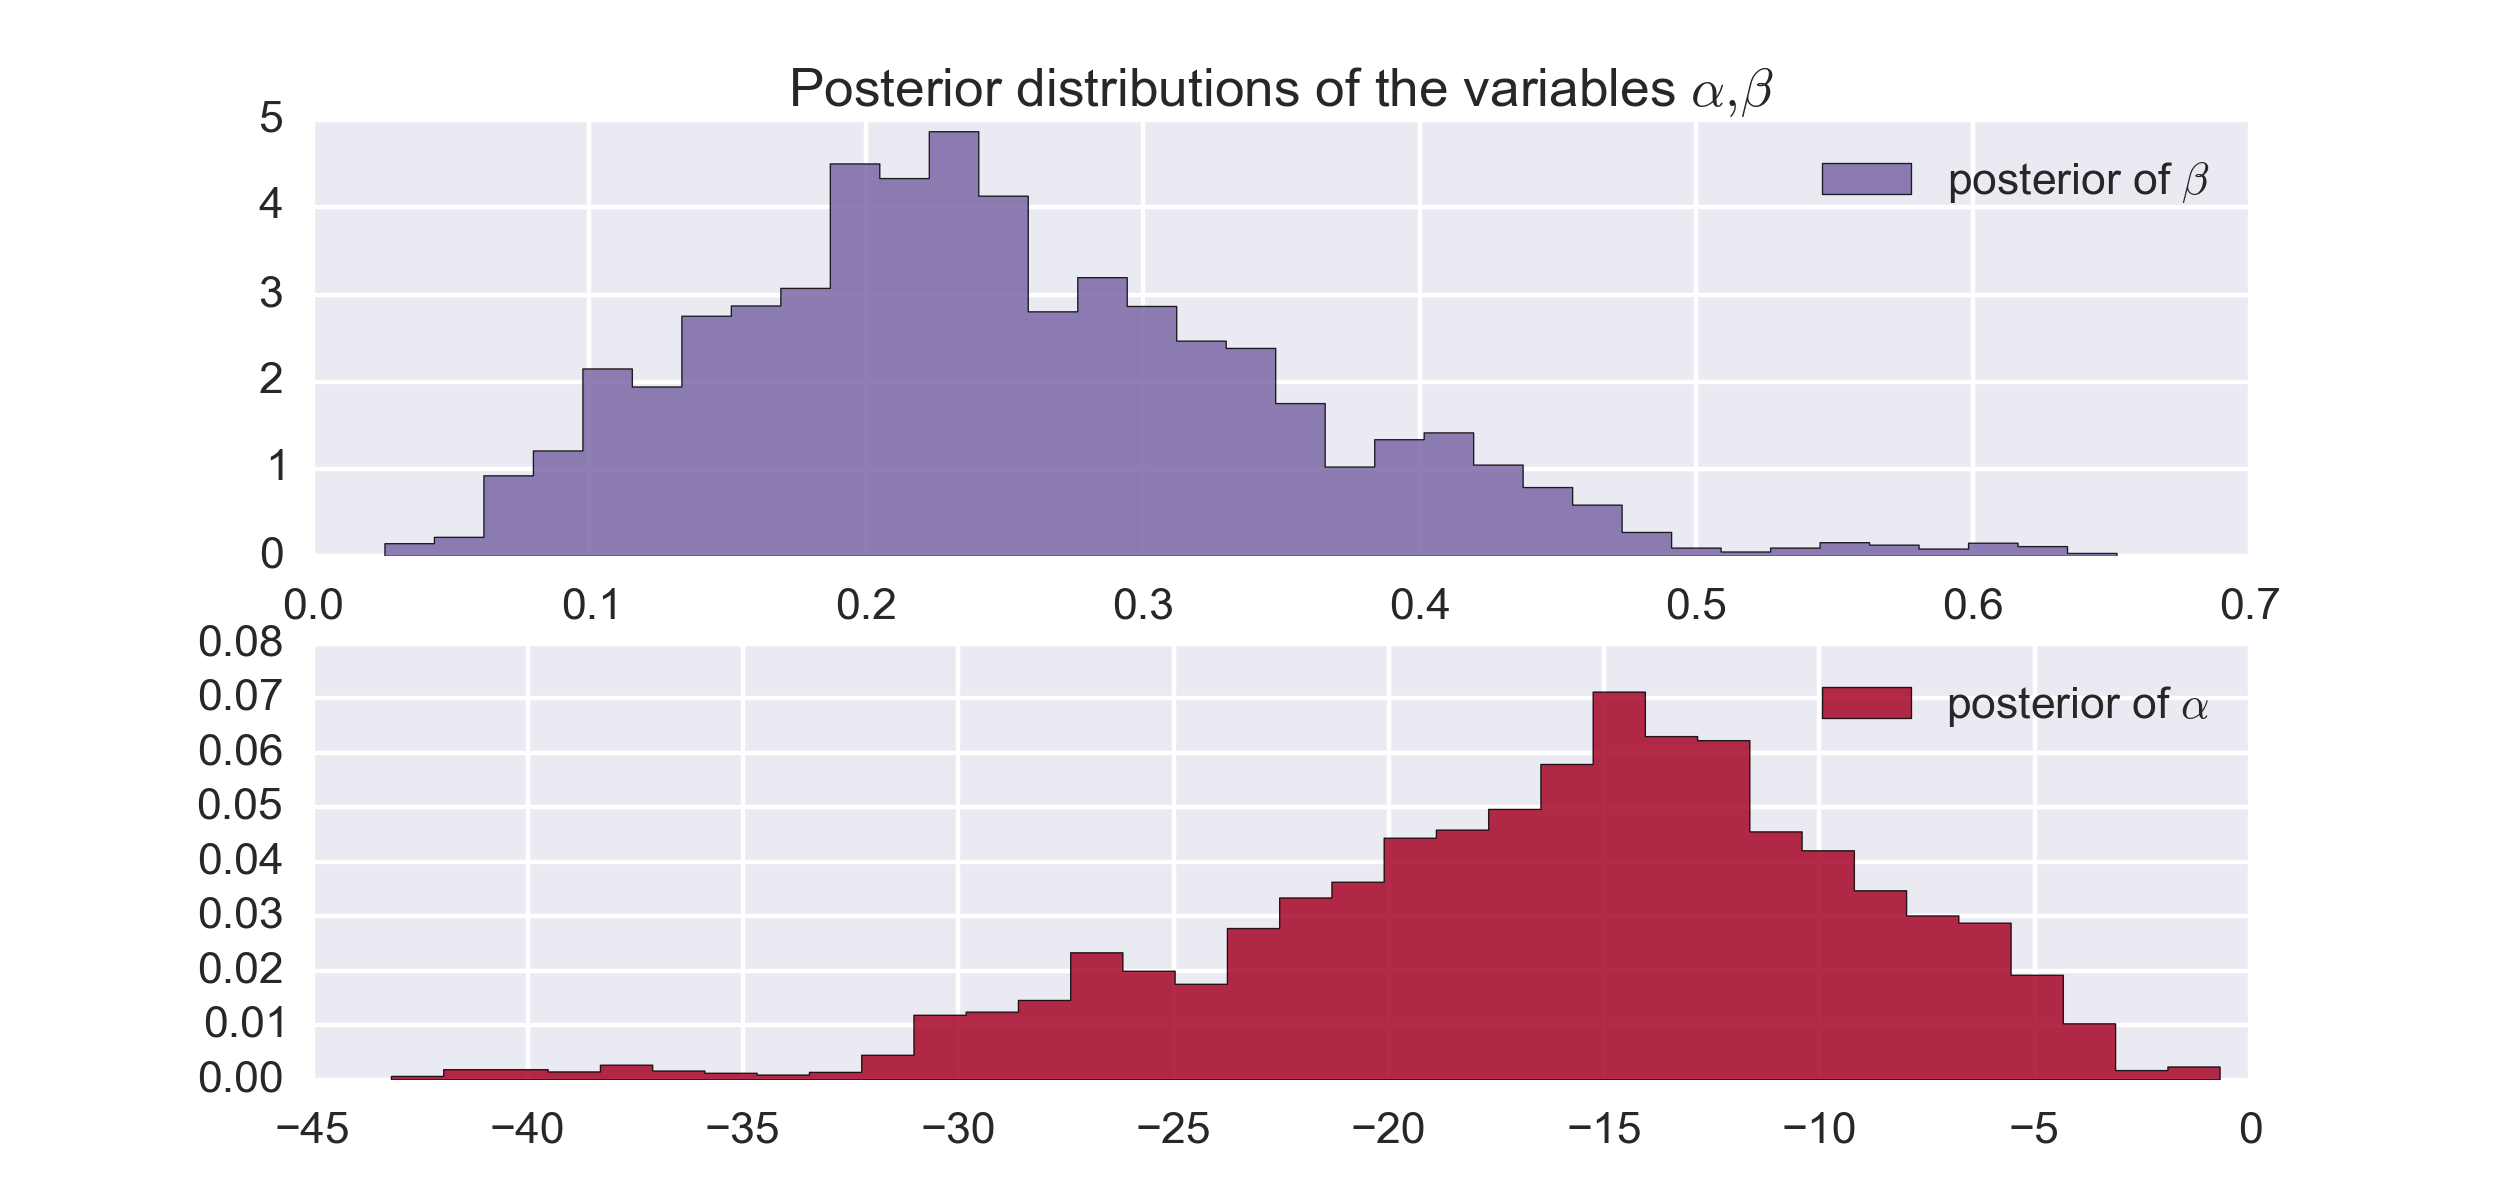
\includegraphics[width=0.75\textwidth]{../Images/Challenger_Parameters.png}\\
  \caption{Probabilities for alpha and beta, from the MCMC simulations.}
\end{figure}

The probability curve for an O-ring failure thus looks as follows:

\begin{figure}[H]
  \centering
  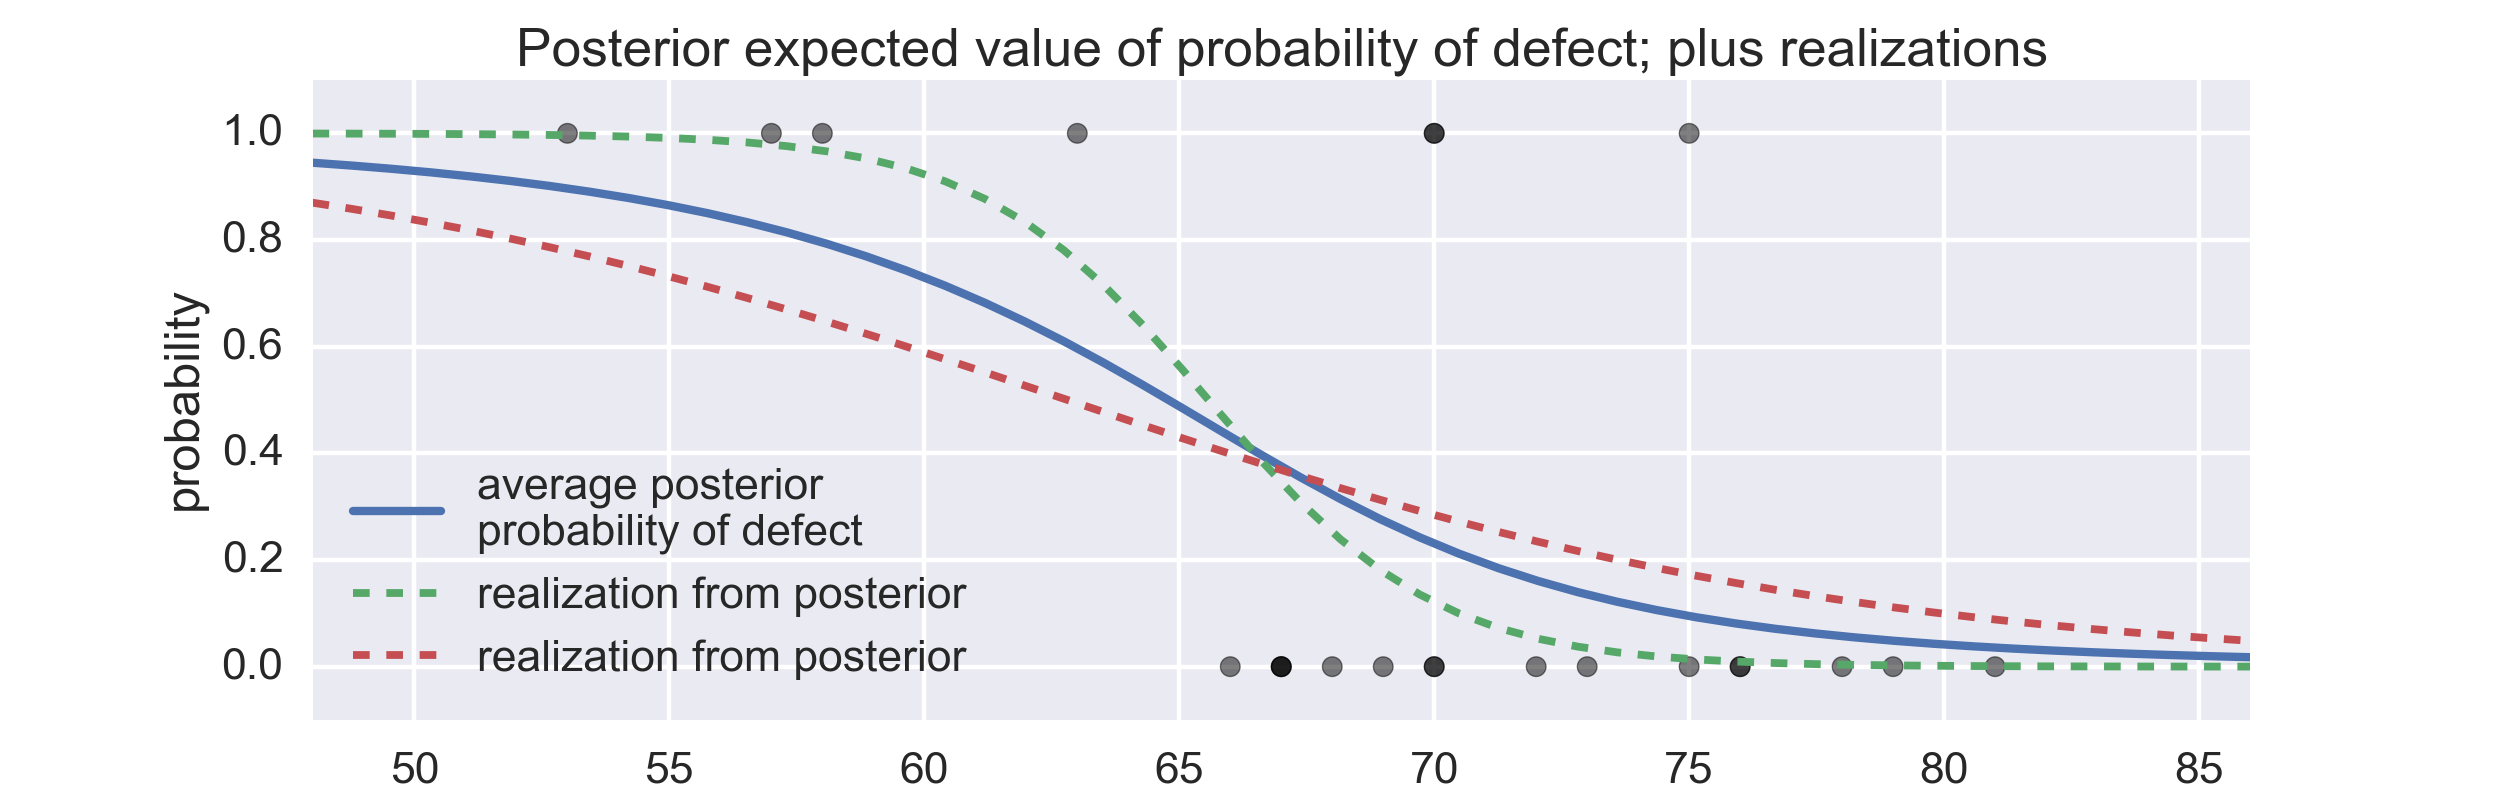
\includegraphics[width=0.75\textwidth]{../Images/Challenger_Probability.png}\\
  \caption{Probility for an O-ring failure, as a function of temperature.}
\end{figure}

One advantage of the MCMC simulation is, that it also provides confidence intervals for the probability:

\begin{figure}[H]
  \centering
  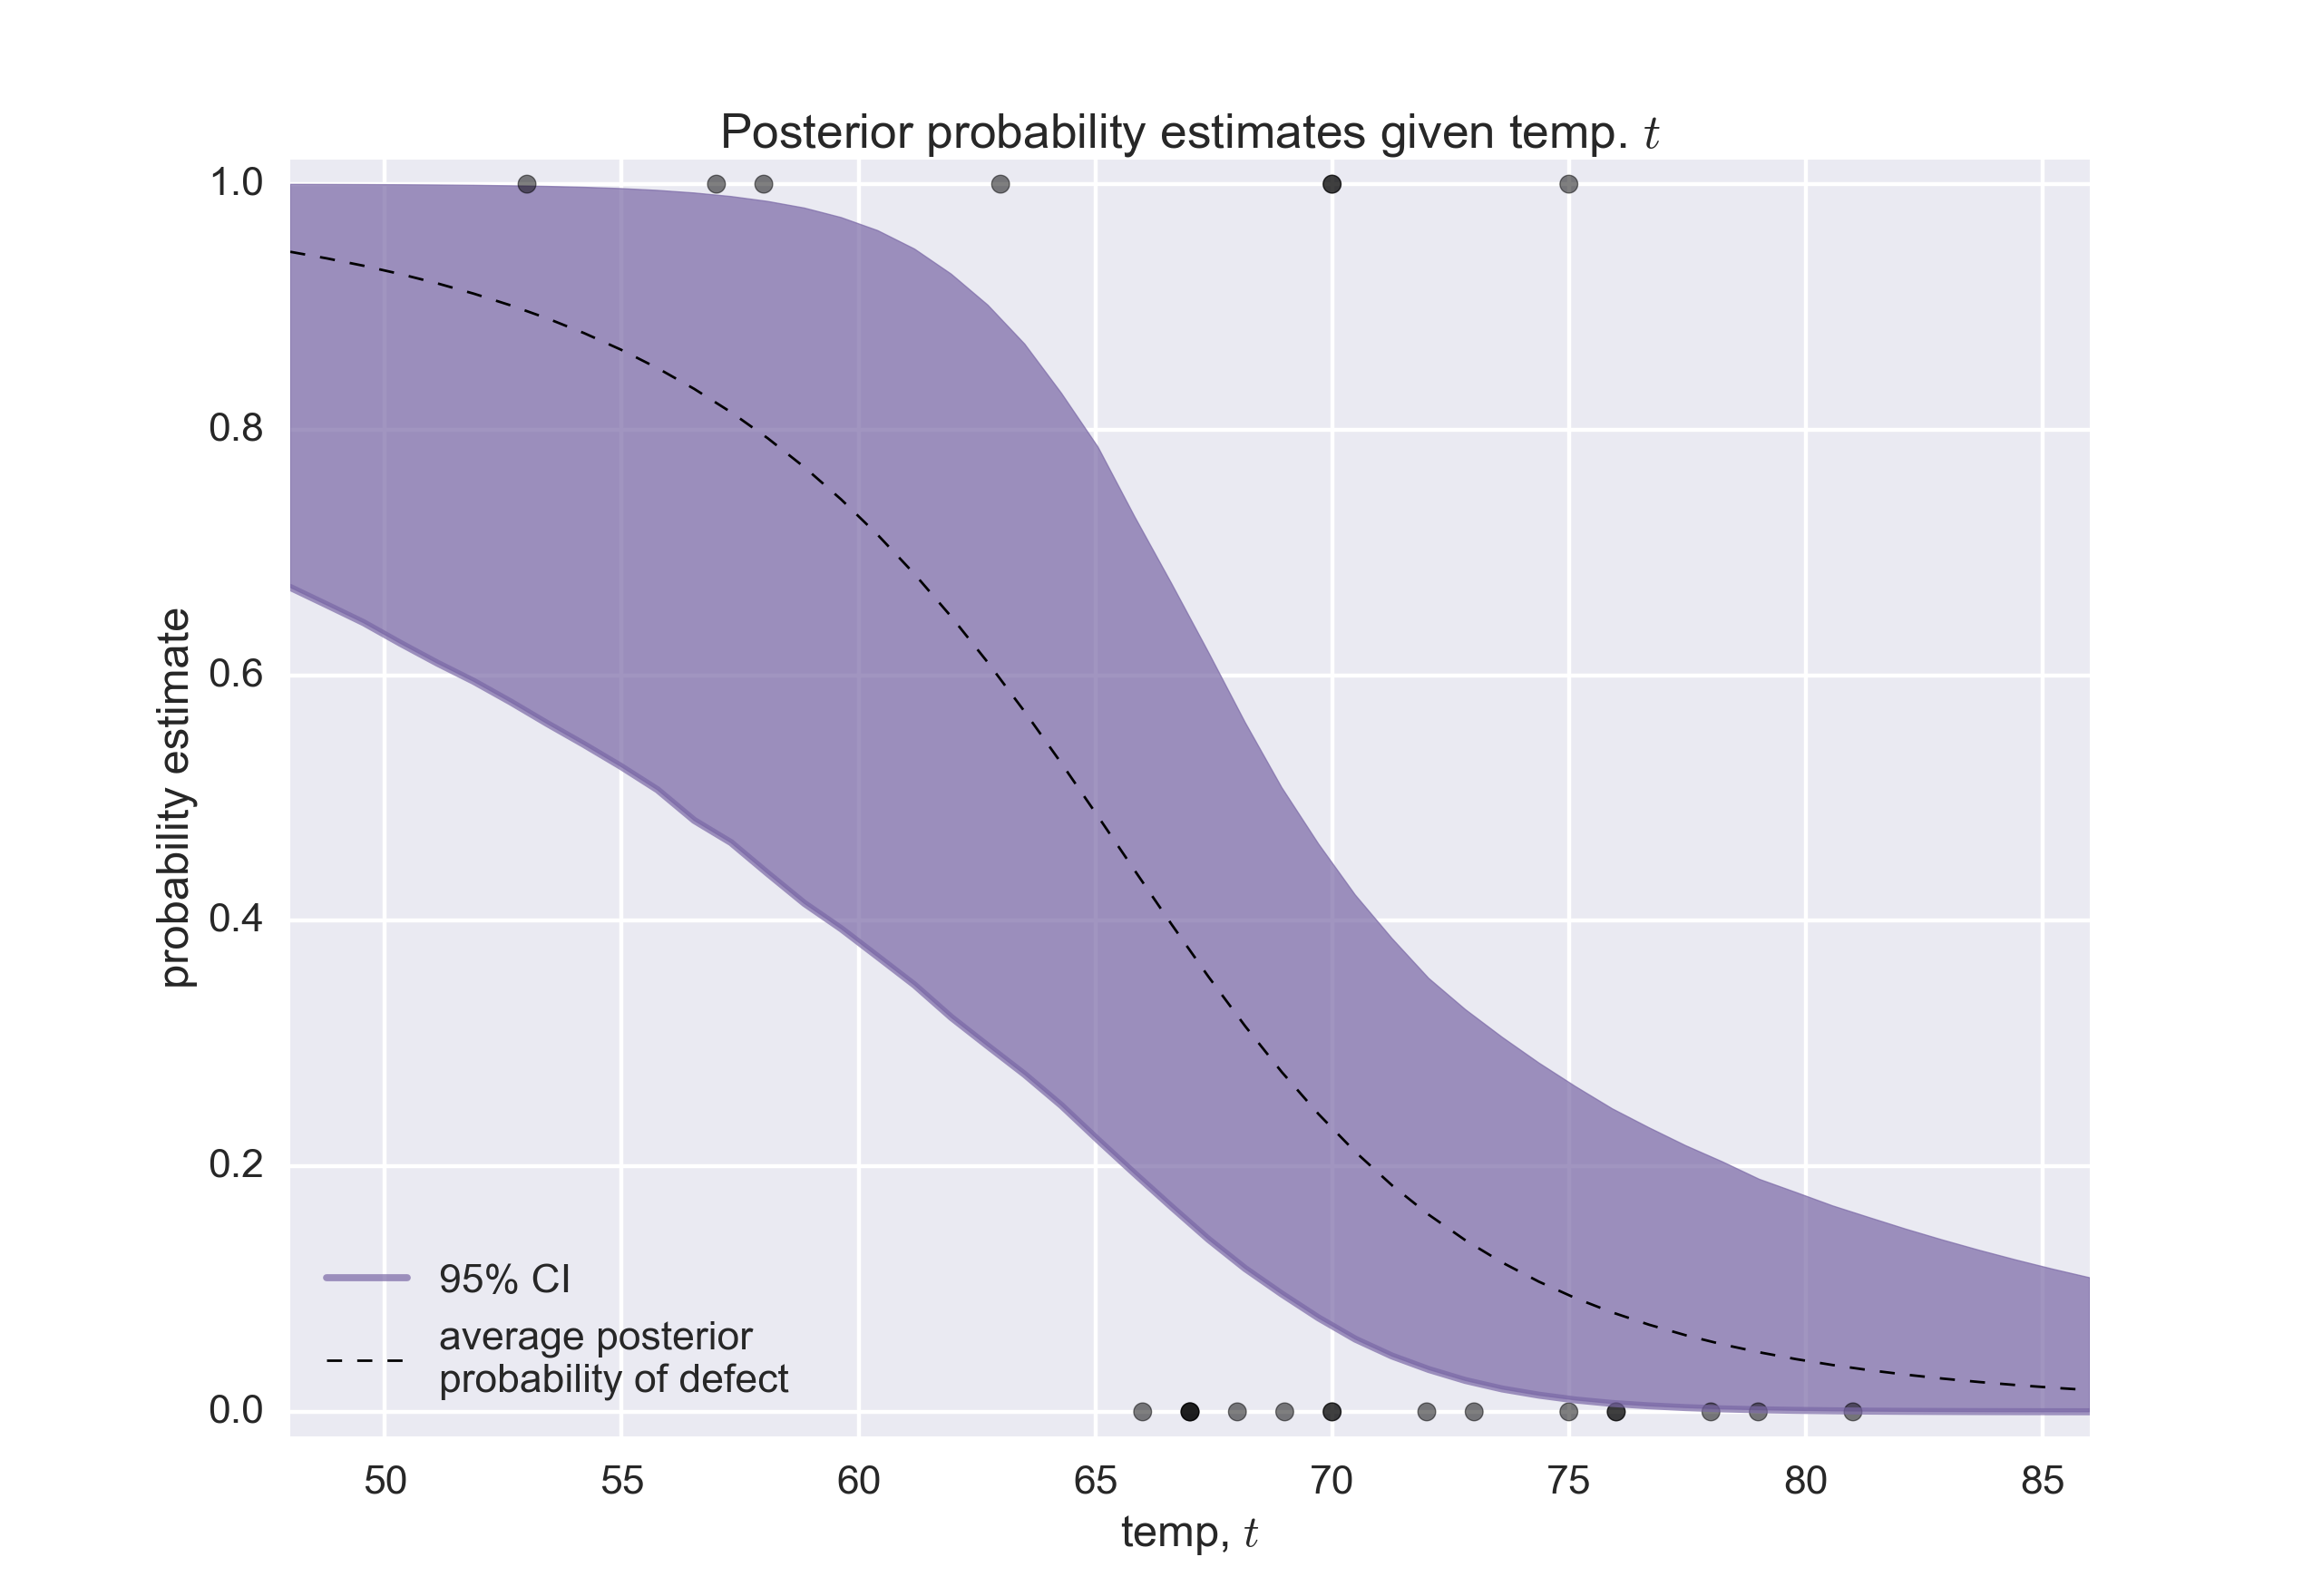
\includegraphics[width=0.75\textwidth]{../Images/Challenger_CIs.png}\\
  \caption{95\% Confidence Intervals for the Probility for an O-ring failure.}
\end{figure}

On the day of the Challenger disaster, the outside temperature was 31 degrees Fahrenheit. The posterior distribution of a defect occurring, given this temperature, almost guaranteed that the Challenger was going to be subject to defective O-rings.

\PyImg "challenger.py" (p \pageref{py:Challenger}): Full implementation of the MCMC simulation. Note that Python 2.x is required for PyMC!.
\index{python}{Bayesian Statistics}

